\documentclass[12pt,preprint]{aastex} 
\usepackage{amsmath, amsfonts, amssymb}

%Remember that in a tex file, a percent sign means 'comment' and the
%rest of the line will not appear in the printed output.

%another option include preprint2, which gives you two columns. to invoke:
%\documentclass[preprint2]{aastex} 

%Note: If you're doing work for some other class and don't want to use
%aastex formatting, you can use some variant of the following commands,
%which are intrinsic to LATEX. However, some commands below, such as
%\altaffiltext and \deluxetable, are peculiar to aastex.

%\documentclass[11pt,a4paper,notitlepage,oneside]{article}
%\usepackage[dvips]{graphicx} 

\begin{document}

\title{YOUR TITLE HERE}

\author{Your Name \\ \today}
%NOTE THE \\ WHICH SKIPS A LINE

\begin{abstract}
Your ABSTRACT here, beginning with broad context of the paper,
moving into finer detail of exactly what your experiment was
testing and why, and culminating with a summary of key findings
and conclusions. Try to quote something quantitative. Aim for
one paragraph, maybe two, and no more.
\end{abstract}

%\tableofcontents

\section{Introduction}
\label{intro} %NOTE THE LABEL SYNTAX

Your INTRODUCTION here. Start with some context and motivation for
your paper, oriented toward, say, a fellow classmate who has not
taken this class yet. Establish why we care, but do not waste time
with grandiose (``Since the dawn of time\dots") statements.

Dial in to the specifics of this paper, what the key concepts are
and what you are going to test.

Finish your intro with a document map: In \S\ref{background} we 
introduce the techniques used in this paper. In \S\ref{experiment1}
we describe \dots and we conclude in 
\S\ref{conclusion}.

\section{Background}
\label{background}

Here is a great place to show us the theory that you learned for
this class (Nyquist Sampling, Fourier Transforms, etc.). Use some
equations.

\begin{equation}
y=mx+b
\label{eq:example}
\end{equation}

Make sure you end your background with a transition into the specific
set up of your first experiment.

\section{Experiment One}
\label{experiment1}

Here you should introduce and summarize the first of your key
experiments for this lab. (You can choose which one that is).
Make sure you are clear on what hypothesis you are trying to test
and what questions you are trying to answer, and how this experiment
is going to test/answer them.

\subsection{Methods / Experimental Setup}

Delve into the specific configuration, setup, and theory for this
experiment that may not have been fully covered in \S\ref{background}.
Feel free to reference previous equations (e.g. ``according to
equation \ref{eq:example}").

Finish this section with a description of the data you collected
(number of samples, time interval, sampling frequency, etc.)

\subsection{Analysis}

Describe the analysis you perform here to extract answers from the
data you collect. Show figures and plots that tell a clear story
and reference them from the text (e.g. ``as Figure \ref{fig:example}
shows, \dots").

\begin{figure}[ht!]
\centering
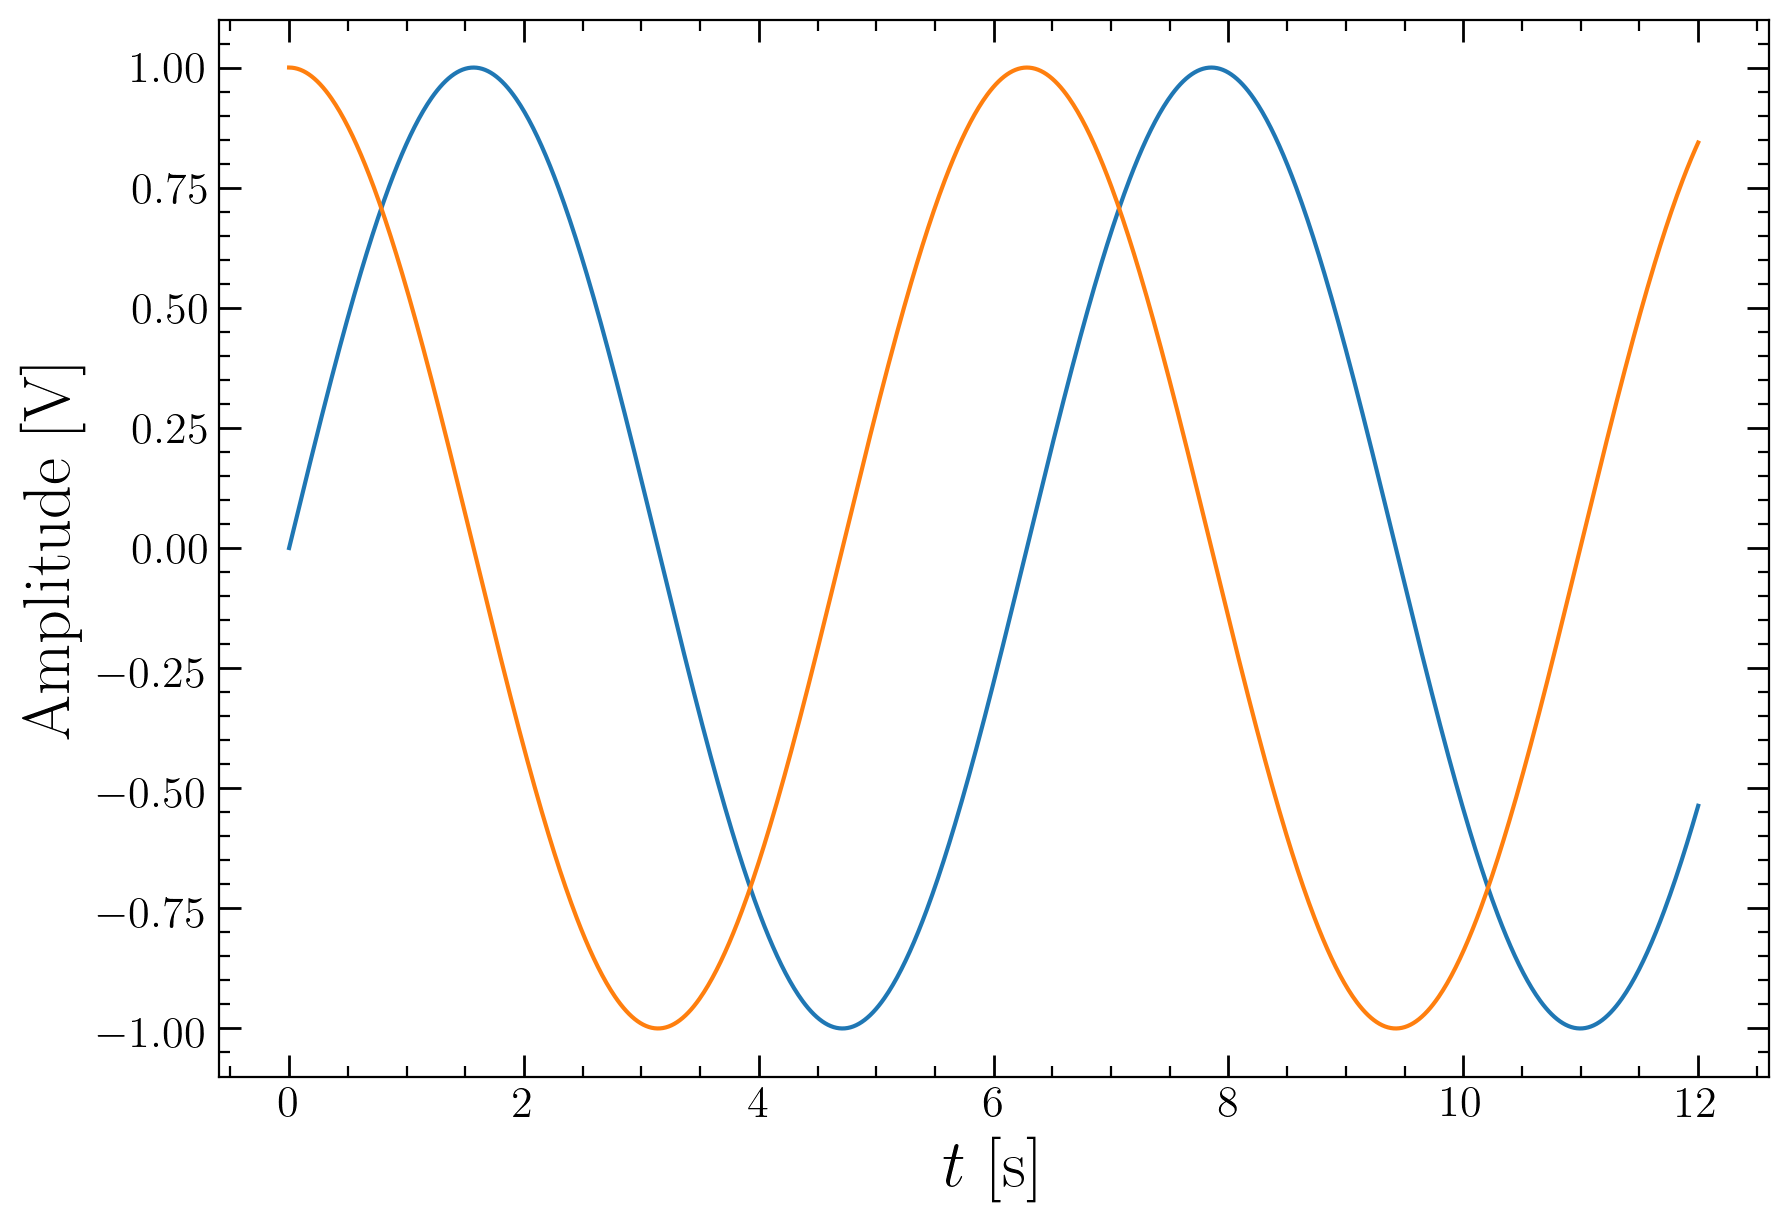
\includegraphics[width=4in]{example.png}
\caption{Write a caption that succinctly summarizes what this plot
is and what the take-away points should be. Aim for three to four
sentences. Make sure your plot has axis labels, a legend, sensible
bounds, and is legible {\it at the default zoom/printing scale}. Note
that \LaTeX has a complicated algorithm for figure placement; it's
okay if your figure is not exactly where you put it in your
text.}
\label{fig:example}
\end{figure}

\subsection{Results}

Here is where you can interpret the analysis in the previous section
to compare what you measured against expectations. Try to make your
comparisons as accurately and quantitatively as possible. Make sure
to answer (or state why the results are not conclusive) your key
questions, but 
do not overstate your findings. Try especially to quantify your
uncertainty.

Measurements with error bars are key results that you should highlight
here. Highlight these results in your abstract, too.

\section{Experiment Two}
\label{experiment2}

\section{Experiment Three}
\label{experiment3}

\section{Conclusion}
\label{conclusion}

Here you should collect and summarize your results. Make sure to highlight the
key points that you found and answer the questions that were asked throughout
the report. Explain how you’ve come to the conclusions that you’re making based
on the results that you’ve presented.

\section*{Acknowledgements}

Here you should acknowledge anyone that helped you with this work (your lab
mates and the division of labor) and software packages used (\texttt{numpy},
\texttt{ugradio}, \texttt{scipy}, etc.). 

\end{document}

Note that anything here is skipped by the interpretor.  You can use it
as scratch paper or to keep templates handy when working on a document. 
Alternately, if you're trying to fix a document with a whole bunch of
bugs in it, temporarily tossing a \end{document} in the middle of the
file will save time, since the compiler won't bother trying to decipher
problems.


